\subsection{Review of \LEGOMOTOR{} Controller Design}

Before starting the final part of our laboratory project, we decided to review the work done in the second assignment. Specifically we wanted to tackle two issues still open:
\begin{itemize}
\item The \textbf{drift} introduced by the \textbf{saturation} block in the signal response to input step functions requesting speed values $\geq{}90\%$ of the maximum speed, as shown in figure \ref{fig:sim_noAW_noSP};

\begin{figure}[H]
\center
  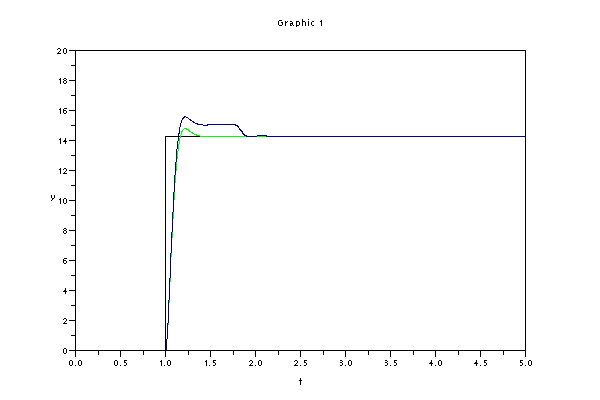
\includegraphics[scale=0.51]{FIGURES_3/Simulation_noAW_noSP.png}
  \caption[SOSModel]{Digital Simulation output: input step signal (black), open loop response (green) and closed loop response (blue)}
  \label{fig:sim_noAW_noSP}
\end{figure}

\item The \textbf{delay} in the motor response detected using the actual data of the \LEGOMOTOR{} with our first implementation of the controller, which was estimated to be around $35ms$;
\end{itemize}

\subsubsection{Anti Wind Up}

When the \textbf{saturation} block constraints the values of the response of the controller, the estimated error may become significant. In fact as time lapses the integral action of the controller becomes more significant but the signal is already saturated. This situation folds itself into a vicious circle that diminishes the system performances, known as ``\textbf{Wind Up}''. 

Common solutions to this problem are:
\begin{itemize}
\item Limitation of the reference signal: by avoiding sharp variations in the input signal (e.g. dividing it's power into a sequence of smaller step functions) the controller's response is less sharp and does not incur into saturation. However this choice degrades system performances;
\item Conditional Integration: by turning off the integrator part in certain conditions (e.g. when signal is saturated and error/control variable have same value) it is possible to avoid increasing the error for a certain amount of time;
\item Back Calculation: when the controller occurs in saturation the integral term is recomputed, so that its action is diminished by a value that is proportional to the saturation action. 
\end{itemize}

We decided to implement the third option in our \textbf{Anti Wind Up} system since it appeared to be more than a hack to just make things work. To do so, the first step has been to compute the \textit{partial fraction expansion} of our digital controller so to isolate its integrating component:

\[
\begin{array}{lcl}
c_1 & = & {8.8625} \over {s} \\
c_2 & = & {-44.8625} \over {80 + s} \\
c_3 & = & 1
\end{array}
\]

Next we apply the bilinear transform to obtain the digital controller components in the \textit{z-plane}:

\[
\begin{array}{lcl}
c_1 & = & {8.8625 + 8.8625q} \over {- 400 + 400q} \\
c_2 & = & {- 44.8625 - 44.8625q} \over {- 320 + 480q} \\
c_3 & = & 1
\end{array}
\]

The next step is to put together the newly find controller components into a scicos circuit, where the integrating part is corrected with the derivative of the error produced by the saturating block. As shown in figure \ref{fig:antiwindup} our new implementation of the \textbf{wheel controller} contains both the old single controller and the new anti wind up system. In figure \ref{fig:sim_yesAW_noSP} it is possible to appreciate the improvement achieved: now the signal overshoot does no more stand to its peak value for some time but it immediately goes toward the desired final value as expected.

\begin{figure}[H]
\center
  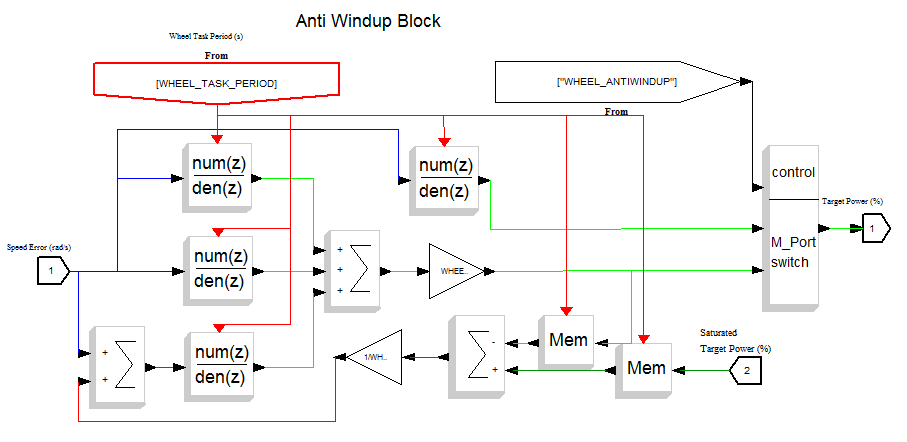
\includegraphics[scale=0.51]{FIGURES_3/Anti_Windup_Block.png}
  \caption[SOSModel]{Scheme of Digital Anti Wind Up Controller}
  \label{fig:antiwindup}
\end{figure}
\large
\begin{figure}[H]
\center
  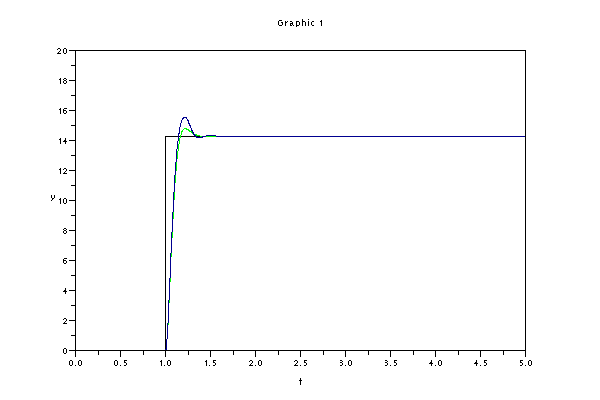
\includegraphics[scale=0.51]{FIGURES_3/Simulation_yesAW_noSP.png}
  \caption[SOSModel]{Digital Simulation output with Anti Wind Up: input step signal (black), open loop response (green) and closed loop response (blue)}
  \label{fig:sim_yesAW_noSP}
\end{figure}

Once verified that the digital simulation worked, the circuit has been implemented in the \textit{LEGO brick}.

\subsubsection{Smith Predictor}

In order to compensate the delay of $35ms$ over the output signal that we detected after the implementation in the actual \textit{LEGO brick}, we decided to use a predictive controller known as \textit{Smith Predictor}.

\begin{figure}[H]
\center
  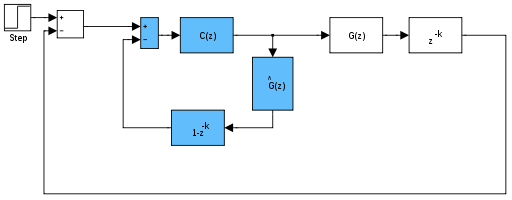
\includegraphics[scale=0.51]{FIGURES_3/smith.png}
  \caption[SOSModel]{Smith Predictor Circuit [source: Wikipedia]}
  \label{fig:smith}
\end{figure}

The \textit{Smith Predictor} circuit is shown in figure \ref{fig:smith}. While the outer loop still feeds the output signal back to the input that is affected by a constant delay effect, an additional inner loop contains the predictor of what the unobservable output of the plant currently is. This circuit has been rearranged into the circuit shown in figure \ref{fig:smith1}.

\begin{figure}[H]
\center
  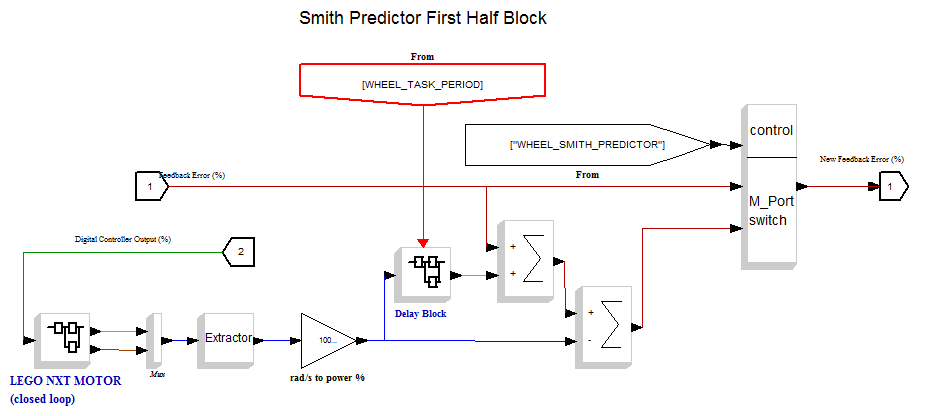
\includegraphics[scale=0.49]{FIGURES_3/Wheel_SmithPredictor_01.png}
  \caption[SOSModel]{Smith Predictor Circuit in Scicos}
  \label{fig:smith1}
\end{figure}

Note that in order to make the simulation work, we had to add a signal delay effect to the feedback data. The circuit that adds the delay is depicted in figure \ref{fig:smith2}.

\begin{figure}[H]
\center
  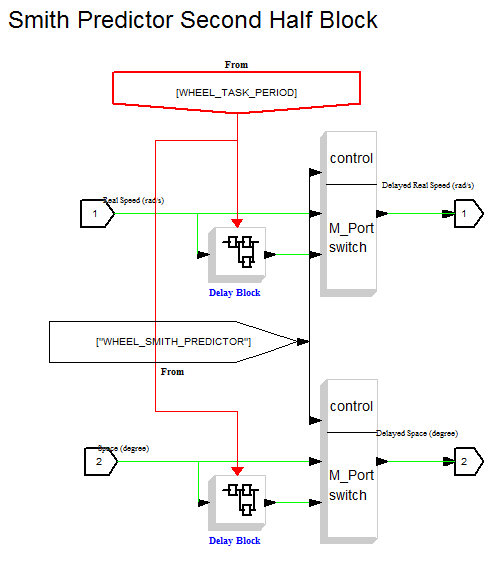
\includegraphics[scale=0.49]{FIGURES_3/Wheel_SmithPredictor_02.png}
  \caption[SOSModel]{Delay Over the signal}
  \label{fig:smith2}
\end{figure}

The output signal obtained using the Smith Predictor is shown in figure \ref{fig:sim_yesAW_yesSP}, where the \textit{blue} signal represents our delayed output signal and the \textit{red} signal stands for the actual output signal that we are able to produce thanks to the predicting controller.

\begin{figure}[H]
\center
  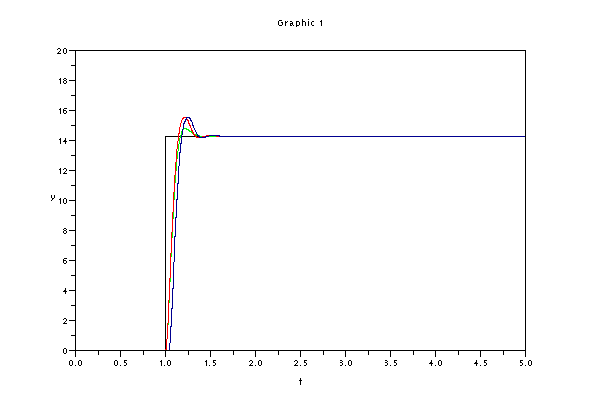
\includegraphics[scale=0.51]{FIGURES_3/Simulation_yesAW_yesSP.png}
  \caption[SOSModel]{Digital Simulation Output with Smith Predictor: input step signal (black), open loop response (green), closed loop response (red) and delayed closed loop response (blue)}
  \label{fig:sim_yesAW_yesSP}
\end{figure}

The final configuration of the Wheel Digital Circuit with the newly added components it is shown inf figure \ref{fig:wheel_circuit}. As it is possible to see, some components already shown in the previous assignment have been encapsulated so that the overall picture could be more clear.

\begin{figure}[H]
  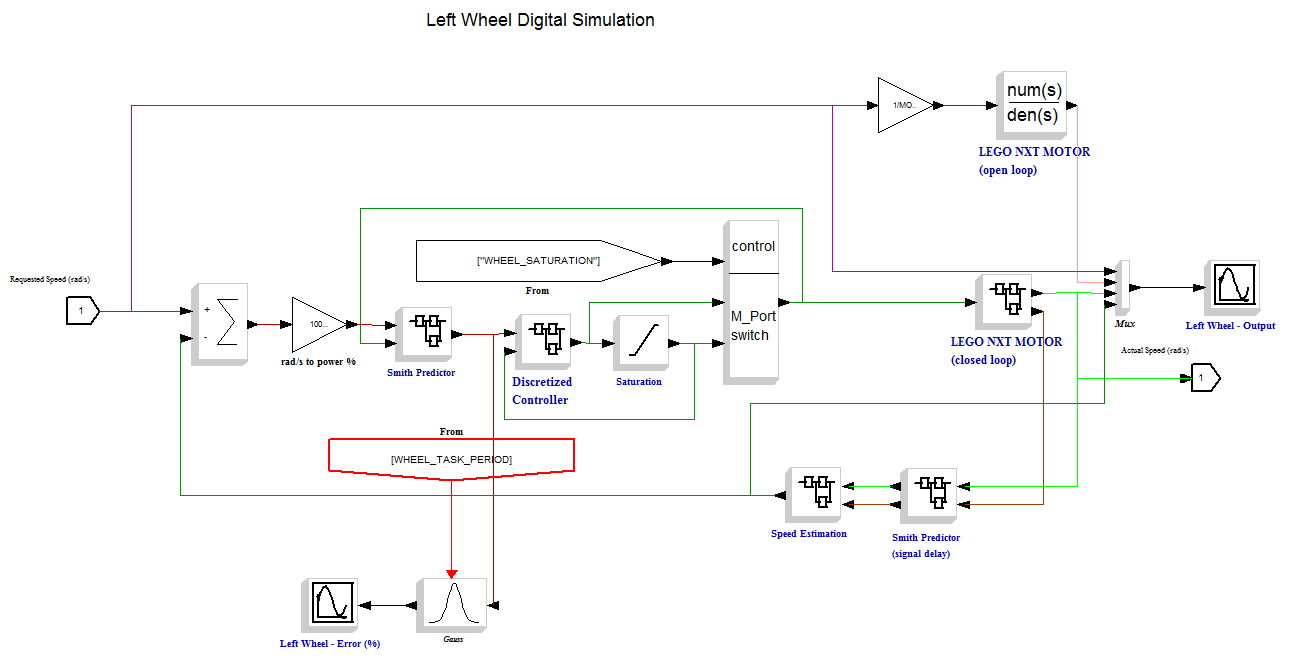
\includegraphics[scale=0.38]{FIGURES_3/Whole_Wheel.png}
  \caption[SOSModel]{Digital Simulation Output with Smith Predictor: input step signal (black), open loop response (green), closed loop response (red) and delayed closed loop response (blue)}
  \label{fig:wheel_circuit}
\end{figure}

\subsection{Unicycle Model}

In this section we will model the behaviour of a \UV{} using the differential drive. A unicycle type robot is in general a robot moving in a 2D world having some forward speed but zero instantaneous lateral motion. In other words it is a \textbf{non-holonomic system}. An example of \UV{} is given in figure \ref{fig:UV model}, where the vehicle is characterized by a couple of parallel driven wheels, with their own motor, and a third small caster wheel.

\begin{figure}[H]
  \begin{center}
  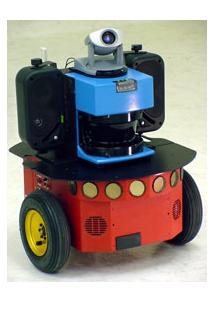
\includegraphics[scale=0.8]{FIGURES_3/unicycle.png}
    \caption[Unicycle Model]{The Pioneer 3-DX8 typical unicycle vehicle}
    \label{fig:UV model}
  \end{center}
\end{figure}

\subsubsection{Kinematic Model}

In order to control and drive this kind of vehicle we need a \textbf{Kinematic Model} that describes the trajectories that the mobile robots follows when subject to commanding speeds. The Kinematic of this system is simple because we have only \emph{non-holonomic} limits. So all the configurations that can be reached by the robot can be described by the vector of coordinates \[ q= \left[
\begin{matrix}
x\\
y\\
\theta
\end{matrix}
\right] \]

\begin{figure}[H]
  \begin{center}
  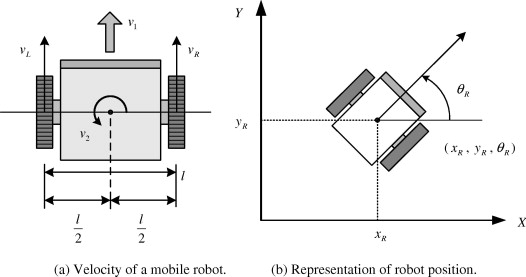
\includegraphics[scale=0.8]{FIGURES_3/kinematic_model.png}
    \caption[Unicycle Model]{The kinematic model of an non holonomic system}
    \label{fig:KM model}
  \end{center}
\end{figure}

In agreement with figure \ref{fig:KM model} the \KM{} can be described by the following non-linear system 
\[\begin{cases}
	\dot x =  v \cos{}\theta{}\\
	\dot y =  v \sin{}\theta{}\\
	\dot \theta = \omega 
\end{cases}
\]
where \emph{v} is the speed of the vehicle and $\omega{}$ is the angular speed of the vehicle.

By knowing that \emph{R} and \textit{L} are respectively the radius of the wheels and the distance between the wheels, we can compute the angular speed of the left and right motor as
$$
\begin{cases}
	v =  \frac{R}{2} (\omega_r + \omega_l)\\
	\omega = \frac{R}{L} (\omega_r - \omega_l)
\end{cases}
$$


\subsubsection{Transfer function of a path following problem}

Since our goal is to follow an imaginary line parallel to the wall we can simplify the Kinematic model by doing some assumptions:
\begin{itemize}
	\item The robot will move forward with a constant speed;
	\item The $X$ axis is parallel to the line that we want to follow;
\end{itemize}
Therefore we obtain the following model:
\[
\begin{cases}
	\dot y =  v \sin{}\theta{}\\
	\dot \theta = \omega 
\end{cases}
\]

It is possible to notice that the kinematic model is non-linear, so we have to linearise it as we want to use a linear controller to control the robot. By using the \textbf{notable limitation}  $\lim_{x\rightarrow 0} \frac{\sin{} x }{x} = 1  $ and assuming that  $\sin{}\theta$ can be approximated by a straight line in contiguous instants (with low values of angular speed $\omega$) we get the desired linear kinematic model:
\[
\begin{cases}
	\dot y =  v \theta{}\\
	\dot \theta = \omega 
\end{cases}
\]

Therefore a first loose approximation of the \textit{transfer function} associated to the vehicle behaviour with our linear kinematic model is given by:
\[
	Y(s) = \frac{V_{speed}}{s^2} U(s)
\]

To improve such an estimation, we may take into account the presence of the wheel engines for which we already computed a transfer function. We aim to find the wheels block contribution to the overall system, hence we look for an input/output relation of type $\omega^\star = G_M(s)\cdot\omega$. We may initially simplify our computations by imposing:

\[
\begin{array}{lcl}
\omega_r & = & \alpha\cdot V_{speed} + \beta\cdot\omega \\
\omega_l & = & \alpha\cdot V_{speed} - \beta\cdot\omega \\
\end{array}
\]

Therefore, provided that $G_r(s)=G_l(s)$ and $\beta = {2\cdot R \over L}$:

\[
\begin{split}
\omega^\star
=&\: G_M(s)\cdot\omega\\
=&\: \left({R \over L}\right)\cdot (G_r(s)\cdot\omega_r - G_l(s)\cdot\omega_l)\\
=&\: \left({R \over L}\right)\cdot (G_r(s)\cdot(\alpha\cdot V_{speed} + \beta\cdot\omega) - G_l(s)\cdot (\alpha\cdot V_{speed} - \beta\cdot\omega))\\
=&\: \left({R \over L}\right)\cdot (2G_r(s)\cdot\beta\cdot\omega)\\
=&\: G_r(s) \cdot \omega\\
\end{split}
\]

So what we have found out is that the contribution of the entire wheel component is actually due only to the closed loop transfer function of such a system, which is $G_r(s)=G_l(s)=G_M(s)=W_{cltf}(s)$:
\[
Y(s) = {W_{cltf}(s)\cdot V_{speed} \over s^2}U(s)
\]

\subsubsection{Estimation of the real distance}

Since we need the distance from the wall we have to use the \emph{NXT ultrasonic sensor} witch is an hardware that can measure distances from some obstacle up to $255 cm$ and with a precision of $\pm 3 cm$.

The ultrasonic sensor is always  perpendicular in respect to the robot and not in respect the wall, therefore when the robot is steering there is an angle $\beta{}$ in respect to the wall that results in a wrong measure of the distance. This problem can compromise the performances of the robot, so it is useful to estimate the orientation of the robot in order to compensate the distance readings obtained from the ultrasonic sensor.

Under the assumption that the robot proceeds along a straight line among subsequent samples taken at intervals of $50ms$, we can use simple trigonometry rules in order to estimate the angle $\beta{}$ in respect to the wall and subsequently compute the real distance $d$. From the configuration of the vehicle shown in figure \ref{fig:TR model} one can derive the following formulas:\\
\[
\begin{array}{lcl}
\Delta{}x &=& v \cdot T_s \\
\beta &=& \arctan \left( \frac{d_{2} - d_{1}}{\Delta{}x} \right) \\
d_{real} &=& \cos(\beta) \cdot d_{2}\\
\end{array}
\]

\begin{figure}[H]
  \begin{center}
  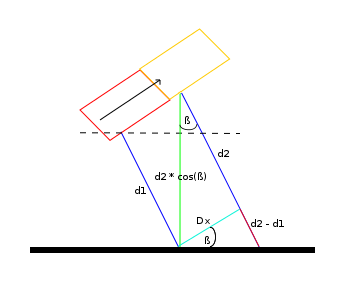
\includegraphics[scale=0.7]{FIGURES_3/estimationAngle2.png}
    \caption[Trigonometry]{Model of the trigonometry used for the estimation of the real distance}
    \label{fig:TR model}
  \end{center}
\end{figure}

\subsection{Vehicle Controller Design}

The vehicle controller design phase retraces the same steps taken for the wheel controller design, thus we will show very briefly all the essential steps without going too much deep into the theoretical details.

\subsubsection{Root Locus}

The \textbf{root locus} will be designed to support a vehicle speed $V_{speed} = 0.34 m/s$, corresponding to $80\%$ of the power that can be given to the motors. This value has been chosen since it leaves ample space for manoeuvre to the additional speed boost caused by the steering behaviour. The desired performances of the \textit{Vehicle Closed Loop System} are given by:
\begin{itemize}
	\item \textbf{Max Overshoot ($O_{max}$)}: $0.01\%$
	\item \textbf{Settling Time ($St_{max}$)}: $5 s$
	\item \textbf{Rise Time ($R_t$)}: $5 s$
	\item \textbf{Overshoot Time ($O_t$)}: $5 s$
	\item \textbf{Steady State Value Tolerance ($\alpha{}$)}: $5\%$
\end{itemize}

Using these values it's straightforward to compute the parameters of the acceptance region, now defined by the values $\omega_n = 0.56$ and $\xi = 0.83$. This time we accept a behaviour that is (a bit) slower than our requirements since we are interested into avoiding too sharp steering behaviours, therefore we consider the inner part of the slice to be our acceptance region.

The \textit{Closed Loop System} transfer function is once again given by:

\[
V_{cltf}(s) = {{V_C(s) \cdot V_P(s)} \over {1 + {( V_C(s) \cdot V_P(s) )}}}
\]

As previously seen, $V_P(s)$ has two possible formulations:
\[
\begin{array}{lcl}
V_{P} &= {{V_{speed}} \over {s^2}} \\
V_{P} &= {W_{cltf}(s)\cdot{}{V_{speed}} \over {s^2}} \\
\end{array}
\]
where $W_{cltf}(s)$ stands for the \textit{Closed Loop System} transfer function of the motor.

In order to get a dominating first order behaviour, that reduces sharp steering behaviours, we add to the root locus a zero in $-0.35$ and a pole in $-2.75$. This time it is not necessary to add poles in zero to obtain zero steady state error tracking, since we already have two. The gain (kc) of the vehicle controller is set to $10$. The final root locus is shown in figure \ref{fig:rlVehicle}, while its analogical formulation is:

\[
		V_C(s) =10\cdot{} {{(s + 0.35)} \over {(s+2.75)}}
\]

\begin{figure}[H]
  \begin{center}
  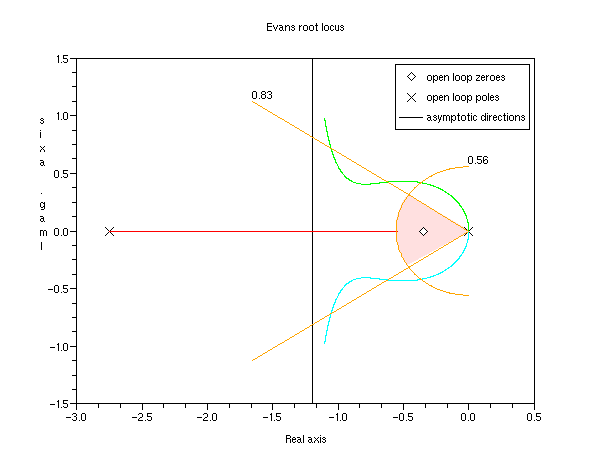
\includegraphics[scale=0.51]{FIGURES_3/VehicleRootLocus01.png}
    \caption[]{Root Locus for the Vehicle Controller with a first order dominating behaviour design}
    \label{fig:rlVehicle}
  \end{center}
\end{figure}

\subsubsection{Digital Model of Vehicle System}

At this stage of the work we are going to create the model that is representing the current situation. The model is always represented by a \textit{Scicos} scheme.

\begin{figure}[H]
  \begin{center}
  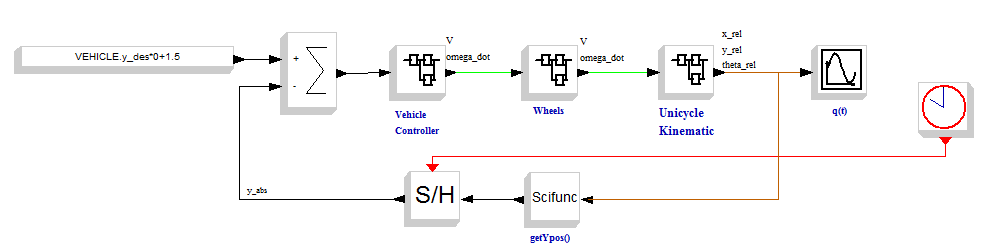
\includegraphics[scale=0.51]{FIGURES_3/Whole_Vehicle.png}
    \caption[]{Complete digital model of the system}
    \label{fig:rlVehicle1}
  \end{center}
\end{figure}

In figure \ref{fig:rlVehicle1} we can see the general vehicle model which contains the vehicle controller, the block of the engines and the block of the kinematic model. This digital model is used to simulate the behaviour of the robot which, with the aid of some \textit{Scipad} functions, can be plotted on the Cartesian plane.
Let's focus on the various blocks in the diagram to understand how the model components work and glue together in the overall picture.

\begin{figure}[H]
  \begin{center}
  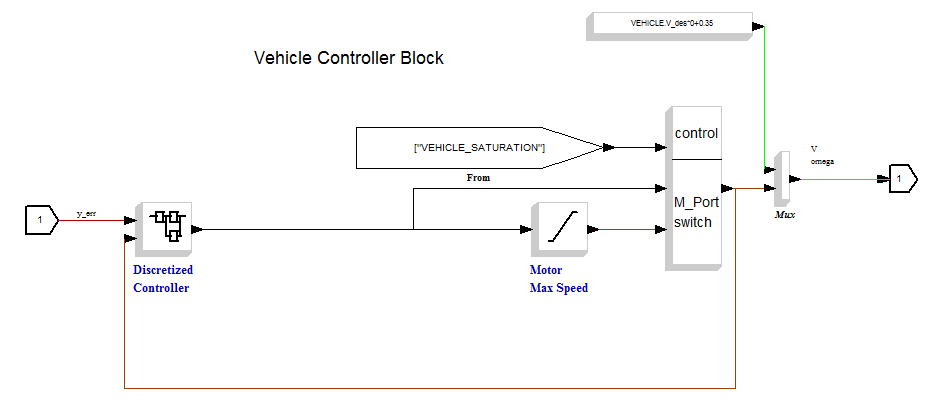
\includegraphics[scale=0.49]{FIGURES_3/Vehicle_Controller.png}
    \caption[]{Controller of the vehicle}
    \label{fig:rlVehicle2}
  \end{center}
\end{figure}

The first component we will drag our attention on is the controller of the vehicle, shown in figure \ref{fig:rlVehicle2}. This super-block contains the actual vehicle controller obtained from the root locus phase and an optional saturation block. The controller receives as input the difference between the desired and the actual distance, while it returns as output the angular speed $\omega_{dot}$ of the vehicle. This value is then combined with the constant forward speed and passed to the wheels.

\begin{figure}[H]
  \begin{center}
  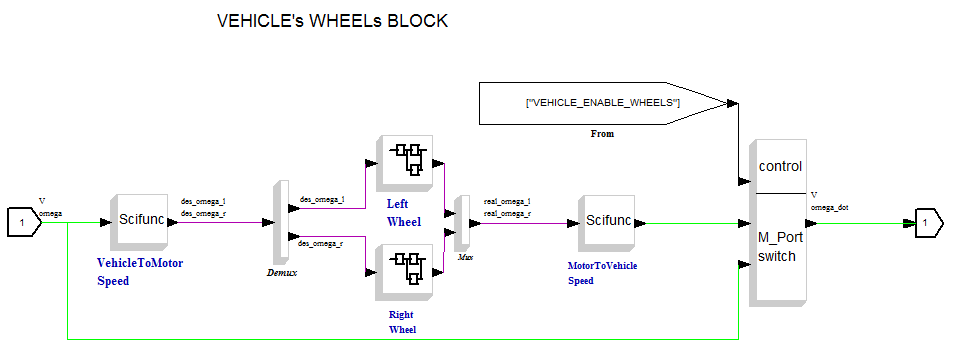
\includegraphics[scale=0.49]{FIGURES_3/Wheels_Block.png}
    \caption[]{Model of the engines}
    \label{fig:rlVehicle3}
  \end{center}
\end{figure}

The second block, shown in figure \ref{fig:rlVehicle3}, simulates the behaviour of a wheel. In this diagram the first component on the left is a function called \textit{VehicleToMotorSpeed} that maps the values of $<v, \omega_{dot}>$ describing the kinematic of the vehicle into the corresponding angular speeds of the wheels. The relation is given by the following equations:

\[
\begin{array}{lcl}
		\omega_l & = & (2\cdot{}v - VEHICLE.rod\_length\cdot{}\omega_{dot})/(2\cdot{}VEHICLE.wheel\_radius);\\
   		\omega_r & = & (2\cdot{}v + VEHICLE.rod\_length\cdot{}\omega_{dot})/(2\cdot{}VEHICLE.wheel\_radius);\\
\end{array}
\]

Since the wheels dynamic is completely transparent from the vehicle point of view, the feedback $<\omega_l, \omega_r>$ obtained by analysing the wheel rotation are then mapped back into the vehicle variables by inverting the previous equations:

\[
\begin{array}{lcl}
v &= &({VEHICLE.wheel\_radius \over{} 2}) \cdot{} (\omega_r + \omega_l)\\
\omega_{dot} &= &({VEHICLE.wheel\_radius \over{} VEHICLE.rod\_length}) \cdot (\omega_r - \omega_l);\\
\end{array}
\]

The internal look of the engine circuit, already shown in figure \ref{fig:wheel_circui}, has been already explained in the part of the report devoted to the wheels controller development and will not be covered here again.

The last component we examine is the Unicycle Kinematic block that takes as input $v$ and $\omega_{dot}$ and computes the values $<x, y, \theta>$ describing the current configuration of the vehicle in the Cartesian space.

\begin{figure}[H]
  \begin{center}
  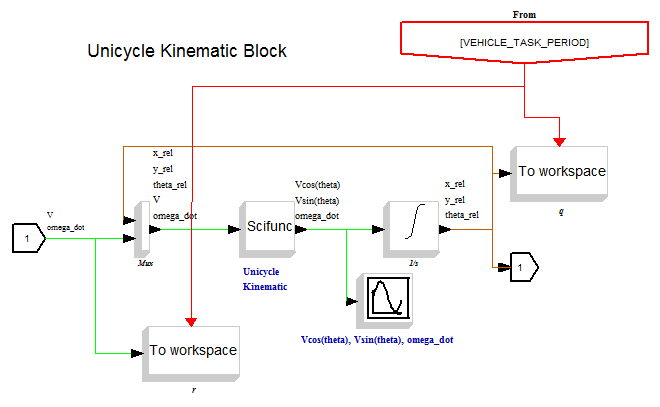
\includegraphics[scale=0.51]{FIGURES_3/Unicycle_Kinematic_Block.png}
    \caption[]{Model of one Unicycle Kinematic Block}
    \label{fig:rlVehicle5}
  \end{center}
\end{figure}

\subsubsection{Vehicle Controller Simulation}

The behaviour of the overall system has been simulated in \textit{Scicos} using both an \textit{analogical} and \textit{digital} circuit. However we will show here only the result of the digital simulation, since it is the most significant data before jumping in the implementation phase. 

Since the \textit{Sonar} can obtain new values at intervals of roughly $30/50ms$ and sometimes it returns spurious data, we decided to keep the controller time period set to $100ms$. This design choice is reinforced by the fact that at worst our wheels block may require up to $135ms$ to stabilize the wheels speed around the desired value. The presence of the speed is completely transparent to our vehicle model, hence we need to maintain the outer loop period big enough so that it is not affected by the feedback loop system of the wheels. Using the \textbf{bilinear transform} we obtain the \textit{z-plane} transform of the vehicle controller:

\[
		V_C(s) =10\cdot{} {{(-0.8637363 + 0.8945055z)} \over {(-0.7582418+z)}}
\]

As it is shown in figures \ref{fig:VeDiSim} and \ref{fig:VePlSim} the overall behaviour of the vehicle respects the imposed requirements. The steering angle of the vehicle is always less than $0.418 rad$, a value for which the linearising simplification of $sin(\alpha)=\alpha$ results in an intrinsic error of $3\%$.

\begin{figure}[H]
  \begin{center}
  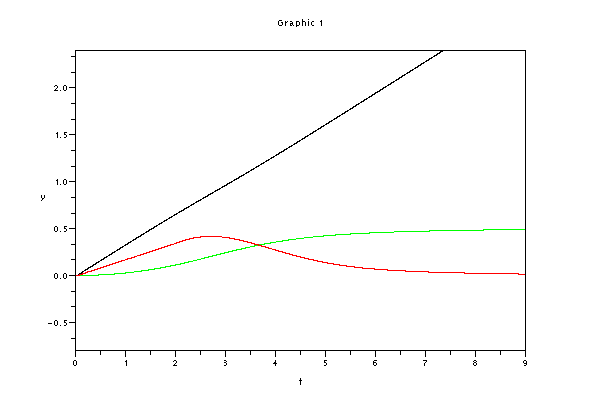
\includegraphics[scale=0.51]{FIGURES_3/VehicleDigitalSim.png}
    \caption[]{Digital simulation output showing the distance from the wall (green), the steering angle computed by the vehicle controller (red) and the covered space (black)}
    \label{fig:VeDiSim}
  \end{center}
\end{figure}

\begin{figure}[H]
  \begin{center}
  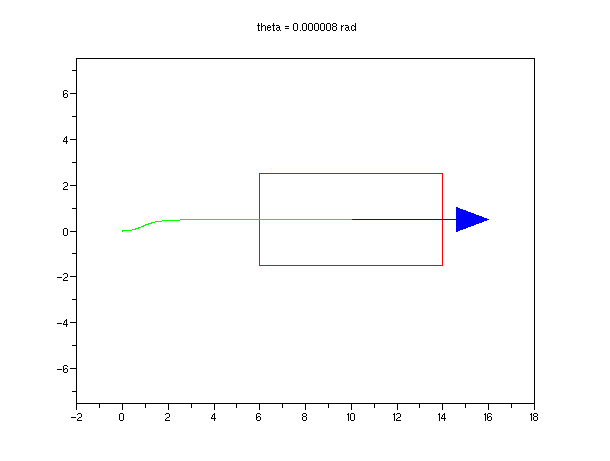
\includegraphics[scale=0.51]{FIGURES_3/VehiclePlotSim.png}
    \caption[]{2D plot of the vehicle behaviour over time}
    \label{fig:VePlSim}
  \end{center}
\end{figure}


\subsubsection{Vehicle Controller Implementation}

The discrete controller function implemented on the Brick has been computed  from the \textit{zeta-transform} of the Controller transfer function with the following steps, in which for simplicity the coefficients have been labelled:

\[
\begin{split}
u(k) =& \: kc \cdot{}  {(e_1 + e_0q) \over (u_1 + u_0q)} \cdot{} e(k)\\
(u_1 + u_0q)\cdot{}u(k) =&\: kc \cdot{} (e_1 + e_0q)\cdot{}e(k)\\
u_1u(k) + u_0u(k)q =&\: kc \cdot{} (e_1e(k) + e_0e(k)q)\\
u_1u(k) + u_0u(k+1) =&\: kc \cdot{} (e_1e(k) + e_0e(k+1))\\
u(k+1) =&\: {kc \cdot{}(e_1e(k) + e_0e(k+1)) - u_1u(k) \over{} u_0}
\end{split}
\]

Since we can not know the future values of the signal, we then applied a change of variable thus obtaining the equation:
\[
u(k) = {kc \cdot{}(e_1e(k-1) + e_0e(k)) - u_1u(k-1) \over{} u_0}
\]

The actual code of the implementation reassembles the one written for the wheels, with the only important difference that now we don't apply any saturation.

\subsection{Performances Tuning and Verification}

This section is devoted to the performance tuning of the vehicle, mainly involving the ultrasonic sensor, and a final review of how the vehicle actually performs when confronting against the real world.


\subsubsection{Tuning of Ultrasonic Sensor}

As it has been outlined in the previous sections, when the vehicle is steering the ultrasonic sensor measurements are affected by an error which is due to the angle of the vehicle moving direction in respect to the wall surface. This problem has been tackled with the aid of a simple triangulation mechanism that appropriately compensates the misreadings.

From time to time the ultrasonic sensor is also affected by spurious saturated measurements that may last even $300ms$, as it is depicted in figure \ref{fig:sonar01}. 

\begin{figure}[H]
  \begin{center}
  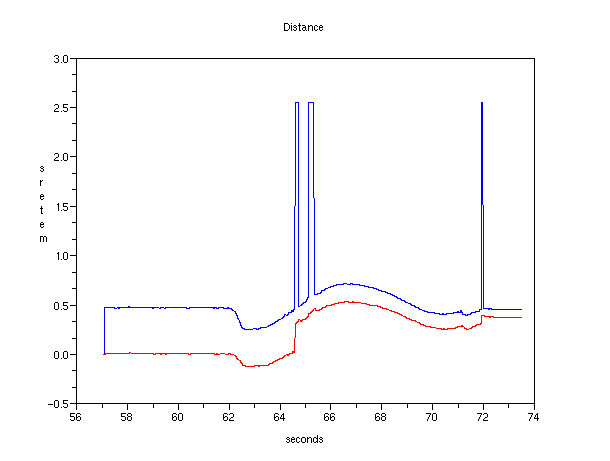
\includegraphics[scale=0.51]{FIGURES_3/Sonar01.png}
    \caption[Trigonometry]{Distance data measured with the ultrasonic sensor (blue) and estimated distance based on feedback speed assuming distance zero as starting position (red)}
    \label{fig:sonar01}
  \end{center}
\end{figure}

Clearly the vehicle can not ground its kinematic over these wrong distance estimations, which make it blind to the real external environment for a certain amount of time. To overcome this problem we decided to implement the kinematic model of the vehicle inside the brick itself, as depicted by the following scrap of code:

\begin{lstlisting}
void unicycle_kinematic(time_data* time)
{
    if ((time->current_time_f - time->start_time_f) < (SONAR_T*2.1)) {
        // At the beginning just use the data coming from the sonar
        oxy_rel.y = sonar_data.cur_estimated_distance;
        oxy_rel.theta = sonar_data.cur_alpha;
    } else {
        // Compute Current Vehicle Speed and Angular Speed
        oxy_rel.vehicle_forward_speed = (vehicle_wheel_radius / 2.0) * (dataA.feedback_speed + dataB.feedback_speed);
        oxy_rel.vehicle_angular_speed = (vehicle_wheel_radius / vehicle_rod_length) * (dataB.feedback_speed - dataA.feedback_speed);
        // Compute new position vector
        oxy_rel.x = oxy_rel.x + (cosf(oxy_rel.theta) * oxy_rel.vehicle_forward_speed * time->delta_time_f);
        oxy_rel.y = oxy_rel.y + (sinf(oxy_rel.theta) * oxy_rel.vehicle_forward_speed * time->delta_time_f);
        oxy_rel.theta = (oxy_rel.vehicle_angular_speed * time->delta_time_f);
    }
}
\end{lstlisting}

Note that the initial conditions of interest of the kinematic model are forcefully loaded from the sonar estimation procedure during the first cycles of activity. Since the digital model depends on data with a certain degree of intrinsic error that accumulates over time, the reference values must be periodically refreshed with the actual data obtained from the ultrasonic sensor. Although this procedure it is not quite sophisticated, it works well and deserves to have its tiny place in this report:

\begin{lstlisting}
void sonar_fun ()
{
    update_timer(&sonar_timer);
    float current_measured_distance = ecrobot_get_sonar_sensor(SONAR_PORT) / 100.0; // meters
    // NOTE: theta estimate within the model is particularly BAD, better use last known angle
    oxy_rel.theta = sonar_data.cur_alpha;
    // NOTE: Every N samples force the simulation to sync to the sonar data
    if ((((int)(sonar_timer.current_time_f*1000)) / ((int)(SONAR_T*1000)) % 20) == 0)
    {
        oxy_rel.y = sonar_data.cur_estimated_distance;
    }
    // Load new Values
    sonar_data.prev_measured_distance = sonar_data.cur_measured_distance;
    sonar_data.cur_measured_distance = current_measured_distance;
    if (sonar_timer.delta_time_f > 0.0) {
        if (sonar_data.cur_measured_distance < 2.40) { // use sonar value
            // Triangulation
            float delta_space = vehicle_target_speed * sonar_timer.delta_time_f; // meters
            sonar_data.cur_error_distance = sonar_data.cur_measured_distance - sonar_data.prev_measured_distance;
            sonar_data.cur_alpha = atanf(sonar_data.cur_error_distance / delta_space); // rad
            sonar_data.cur_trigon_distance = (float) (sonar_data.cur_measured_distance * cosf(fabsf(sonar_data.cur_alpha)));
            // Prepare for Filtering
            mem_dist_sonar[mem_sonar_index] = sonar_data.cur_trigon_distance;
            mem_time_sonar[mem_sonar_index] = sonar_timer.delta_time_f;
            mem_sonar_index = (mem_sonar_index + 1) % MEM_SONAR_LENGTH;
            // Apply Filtering
            sonar_data.cur_filtered_distance = moving_average_vector(mem_dist_sonar, mem_time_sonar, MEM_SONAR_LENGTH);
            // Choose one value
            sonar_data.cur_estimated_distance = sonar_data.cur_filtered_distance;
            // Update the Unicycle Kinematic Model
            unicycle_kinematic(&sonar_timer);
        } else { // Use simulation instead of sonar
            // Last computed distance should be reliable more or less
            oxy_rel.y = sonar_data.cur_estimated_distance;
            // Apply Unicycle Kinematic to predict distance according to model
            unicycle_kinematic(&sonar_timer);
            sonar_data.cur_estimated_distance = oxy_rel.y;
            sonar_data.cur_measured_distance = oxy_rel.y; // WARNING: approximation with tiny error
        }
    } else {
        sonar_data.cur_estimated_distance = current_measured_distance;
    }
}
\end{lstlisting}

The procedure starts with an initialization phase that updates the values of the timer associated to the sonar, takes the sonar distance and periodically synchronizes the kinematic model with the measured distance. If the ultrasonic sensor does not return potentially wrong distance measurements, we correct the distance estimates using the triangulation rules and apply a moving average filter of size $5$. Otherwise we forcefully update the kinematic model with the last good estimate of the distance and use it to compute the new distance.

In figure \ref{fig:sonar02} are shown the various (intermediate) distance estimations available to the robot collected during one of many experiments. The \textit{blue} line stands for the actual measurements collected with the sonar, the \textit{red} line results from the triangulation procedure while the \textit{green} one results from the filtering. In this plot its not easy to spot when the sonar misread the distance, since in such a case the measured values are always overridden using the kinematic model that is the \textit{black} line. As you can see the triangulation introduces a slight oscillation in its output values that is probably an error due to the usage of trigonometric functions, while from time to time introduces an instantaneously significant error that is by the way filtered out by the moving average.

\begin{figure}[H]
  \begin{center}
  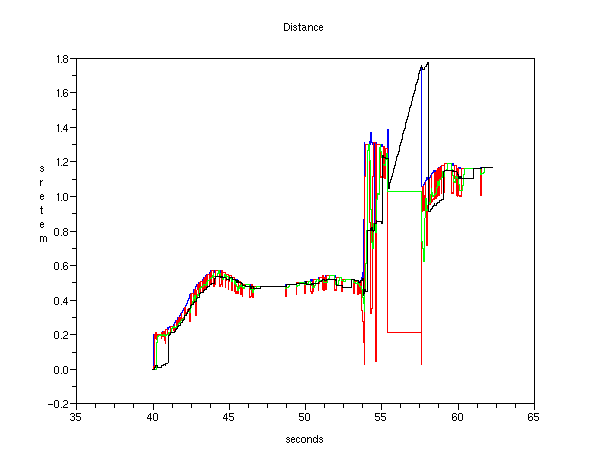
\includegraphics[scale=0.51]{FIGURES_3/Sonar02.png}
    \caption[Trigonometry]{Distance measurements}
    \label{fig:sonar02}
  \end{center}
\end{figure}

Near the time of $54s$ the vehicle incurred into the end of the wall, hence it initially measured the new distance but as time went by it lost the wall reference for a few seconds due to the particular angle that the vehicle had in respect to the wall, which caused the ultrasonic wave to not be reflected back. Luckily the vehicle controller can recover from this particular situation by steering toward the reference wall. If the wall is actually there and the vehicle did not turn too much, then after some time it will follow the path after the corner, otherwise it will end up looping in a circle. The latter situation is the worst case example and can not be theoretically avoided with the limited instruments and sensors we have been provided for this project.

\subsubsection{Turbo Boost}

Since our vehicle is configured to proceed at a relatively modest speed, which is $0.337 m/s$, we decided to provide it with a \textit{Turbo Boost} utility. This utility increases the general speed of the vehicle when it is following the wall at the right distance and with a nearly zero angle. This task is accomplished by the following simple piece of code:

\begin{lstlisting}
    // Turbo Boost Facility
    if ((fabsf(sonar_data.cur_alpha) < 0.01)  && (fabsf(sonar_data.cur_estimated_distance - WALL_DISTANCE) < 0.035))
    {
        vehicle_target_power = 95; // %
    } else {
        vehicle_target_power = TARGET_POWER; // 80%
    }
    vehicle_target_speed = ((k * input_power * vehicle_target_power * vehicle_wheel_radius) / 100.0);
\end{lstlisting}

\subsubsection{Overall Observations}

When the vehicle starts up to $0.5m$ far away from the desired path but parallel to the wall, as it was the case for the measurement data shown in figure \label{fig:sonar02}, it is able to reach the desired distance from the wall within $5-6s$. These performances are acceptable both in respect to the outcome of the digital simulation in \textit{Scicos} and to our initial requirements.

The vehicle can also start with an initial angle that is up to $45$ degrees in respect to the wall, in which case it obviously requires more time to converge. In our experimentations the vehicle performed better when it was initially placed near the wall rather than far from it, probably due to the fact that in the latter case the ultrasonic measure uncertainty connected to the angle in respect to the wall is bigger.

Although the vehicle immediately reacts to obstacles placed in front of the wall, their length must be of at least $1.5$ meters in order to let the vehicle approach the new reference path given the high speed it is moving forward.
